\documentclass{article}
\usepackage[utf8]{inputenc}
\usepackage{graphicx}
\usepackage{hyperref}
\usepackage{float}
\usepackage[export]{adjustbox}

\title{Proof Of Concept Design}
\author{Sophie Wallace }
\date{September 2019}

\begin{document}

\maketitle
\tableofcontents
\clearpage

\section{Introduction}
This Proof of Concept (PoC) design draws from extensive scoping and testing conducted in tasks Scoping II, Elaboration I and II. These tasks sought to identify appropriate tools and techniques necessary to solve the pains that are frequently experienced in anthropological fieldwork. Through these tests, I established the most significant gain creator would be a technology that assists with organising and storing data from the field including notes, images, audio and video. Additional features of this tool will be discussed further in the user stories.  


\section{User Stories}
A user story is a method to add business value by capturing requirements from user perspective in the form of some description (SYSTANGO 2019). User stories are vital in understanding the features that users value and prioritise. For this PoC, user stories will address the required features for this PoC to be eventually demonstrated. \textbf{Figure 1} displays the concept of the 3 Rs needed for a contextual and concise user story (SYSTANGO 2019).

\begin{figure}[H]
    \centering
    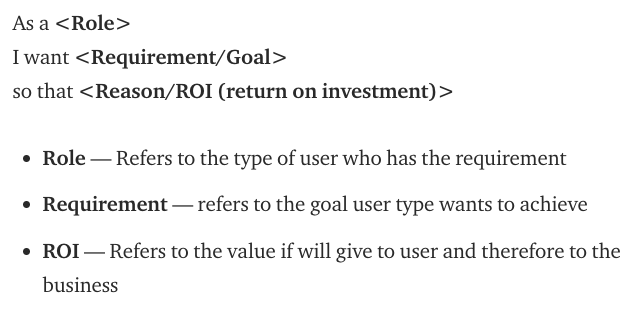
\includegraphics[width=\textwidth, frame]{UserStories_ThreeRs.png}
    \caption{3 Rs of User Stories}
    \label{fig:my_label}
\end{figure} 

For each of the user stories provided below, acceptance criteria will then follow. This aims to articulate exactly when the user story is done from product owners perspective to produce acceptance tests (SYSTANGO 2019). As this technology is targeted to assist with ethnographic data management, each user story will be from the perspective of an anthropologist.
\clearpage



\section{User Stories in Ethnography}    
\begin{itemize}
\item As an anthropologist, I want the data collected on my mobile to be transferred to my laptop so I can have a streamlined process for data collection and storage.
\item As an anthropologist, I want all of my ethnographic data types such as text, photos, video and audio, to be organised in one space so I can organise large data sets and save time locating data.
\item As an anthropologist, I want all my collected data to have rich metadata and be tagged so I can conveniently identify the defining features of each data type. 
\item As an anthropologist, I want to be able to edit text data types so I can add, adjust and refine collected data in one organised space.
\item As an anthropologist, I want data management to function offline so I can avoid depending on internet connection.
\item As an anthropologist, I want to be able to store collected data in an external system so I can ensure all materials are secure and backed up.  
\end{itemize}

\section{Themes and Categories}
Upon examination, each user story has a clear theme and category necessary for this POC design. These include:
\begin{itemize}
    \item Mobile and desktop compatibility
    \item Data type compatibility
    \item Metadata management
    \item Editing text documents
    \item Offline function
    \item Secure storage system
\end{itemize}

In identifying these categories, it is essential to understand how they depend on each other and whether there are prerequisites to their functioning. The stories that \textbf{must} be completed first include:
\begin{enumerate}
\item Data type compatibility
\item Metadata management
\item Secure storage system
\end{enumerate}
Thereafter, the additional features such as mobile and desktop compatibility, editing text documents, and offline functioning \textbf{might} be completed to enhance the eventual POC demonstration. 

\section{Acceptance Criteria}
Acceptance criteria involves articulating tests to ensure the user stories are completed or not completed. This is a quality assurance practice to verify if the acceptance criteria covers what's been expected (SYNTAGO 2019). The following tests aim to articulate tests that will identify whether these user stories have been met. 

\subsection*{Mobile and Desktop Compatibility}
As an anthropologist, I should be able to:
\begin{enumerate}
\item Collect data on my mobile
\item Upload the data onto the technology
\item Access this technology on my desktop
\item Access the mobile uploaded data 
\end{enumerate}

\subsection*{Data Type Compatibility}
As an anthropologist, I should be able to:
\begin{enumerate}
\item Upload all data types to the technology
\item View each data type 
\end{enumerate}

\subsection*{Metadata Management}
As an anthropologist, I should be able to:
\begin{enumerate}
\item Open data type
\item Add name, date, type, location, persons and description as metadata
\item Tag data to categorise data sets into type
\end{enumerate}

\subsection*{Editing Text Documents}
As an anthropologist, I should be able to:
\begin{enumerate}
\item Open text data type
\item Access editing format
\item Edit document
\item Save edited document
\end{enumerate}

\subsection*{Offline Function}
As an anthropologist, I should be able to:
\begin{enumerate}
\item Enter the technology without internet access
\item Upload data without internet access
\item Edit and manage data without internet access
\end{enumerate}

\subsection*{Secure Storage System}
As an anthropologist, I should be able to:
\begin{enumerate}
\item Save all data types in single system
\item Sync all data into external storage
\item Access control mechanism in storage
\item Implement tiered security system in storage
\item Be protected from software virus'
\end{enumerate}


\section{References}
SYSTANGO. 2019. “working ” Medium. Medium. January 11, 2019. \.Perkel, Jeffrey M. 2019. “Workflow Systems Turn Raw Data into Scientific Knowledge.” Nature 573 (7772): 149–50. https://doi.org/10.1038/d41586-019-02619-z

\end{document}
